\documentclass[12pt]{basque-book}
\usepackage[a4paper]{geometry}
\usepackage[myheadings]{fullpage}
\usepackage{fancyhdr}
\usepackage{lastpage}
\usepackage{graphicx, wrapfig, subcaption, setspace, booktabs}
\usepackage[T1]{fontenc}
\usepackage[font=small, labelfont=bf]{caption}
\usepackage{fourier}
\usepackage[protrusion=true, expansion=true]{microtype}
\usepackage[basque]{babel}
\usepackage{sectsty}
\usepackage{url, lipsum}
\usepackage{graphicx}
\usepackage[utf8]{inputenc}
\usepackage{courier}
\usepackage{ulem}
\usepackage{spverbatim}
\usepackage{multirow} %para las tablas
\usepackage{color}
\usepackage{graphicx}
\usepackage{epsfig}
\usepackage{multirow}
\usepackage{colortbl}
\usepackage{xcolor}
\usepackage{float}
\usepackage{fancyvrb}
\usepackage{bera}
\usepackage{adjustbox}
\usepackage{amsmath}


\usepackage{listings} %For code in appendix


\newcommand{\HRule}[1]{\rule{\linewidth}{#1}}
\onehalfspacing
\setcounter{tocdepth}{5}
\setcounter{secnumdepth}{5}

%-------------------------------------------------------------------------------
% HEADER & FOOTER
%-------------------------------------------------------------------------------
\pagestyle{fancy}
\fancyhf{}
\setlength\headheight{15pt}
\fancyhead[R]{\MakeUppercase{matematika diskretua}}
\fancyfoot[C]{\thepage}
%-------------------------------------------------------------------------------
% TITLE PAGE
%-------------------------------------------------------------------------------

\begin{document}

\title{ \textbf{Matematika Diskretua\\ RSA Kriptografia Txostena} }

\author{Xabier Garrote}

\date{\today a}


\maketitle
\newpage
\tableofcontents
\newpage


%--------------------------------------------------------------------% Documentuaren atalak ezberdinak hemendik aurrera ---------------------------------------------------------------------
\chapter{Sarrera}
Euskaltzaindiaren arabera \textbf{kriptografia} "\textit{Ezkutuko kodeen bidez idazteko modua}" da. Hau da, mezu baten edukia igorleak eta hartzaileak \textbf{bakarrik} irakurtzeko kriptografia erabiltzen da.
\\
Igorleak mezua bidaltzean zifratu egiten du. Hartzaileak mezua jasotakoan deszifratu, egiten du irakurri ahal izateko. 
\\

Historian zehar hainbat kriptografia sistema ezberdin erabili dira.
\begin{itemize}
    \item Espartanoek K.a. V mendean mezuak ohial baten gainean idazten zituzten. Mezua zifratzeko ohiala loditasun jakin bateko makil baten gainean inguratzen zuten. Ondoren, mezua idazten zuten eta hartzaileari bidali. Hartzaileak mezua jasotzean igorlearen loditasun bereko makil batez baliatuz bertako edukia irakur zezakeen.
    
    
    \newpage
    
    
    \item Polybiosen zifratze-sistema K.a II mendean sortutakoa. 
    \begin{center}
        \begin{tabular}{ c |c |c| c| c| c| }
            & \textbf{A}  & \textbf{B} & \textbf{C} & \textbf{D} & \textbf{E} \\
             \hline
            \textbf{A}  &a  & b & c & d & e \\ 
            \hline
            \textbf{B}  &f  & g & h & i/j & k\\  
            \hline
            \textbf{C}  & l  & m & n & o & p \\
            \hline
            \textbf{D}  & q  & r & s & t & u\\
            \hline
            \textbf{E}  & v  & w & x & y & z
        \end{tabular}
    \end{center}
    
    Letra bakoitza matrizean duen kordenadengatik ordezkatzen da. Adibidez, \textbf{a} letra \textbf{AA} izango litzateke, \textbf{q} letra \textbf{DA} eta abar.
    
    Zifratze sistema hau 25 karakterentzako pentsatuta dago, beraz, guk erabiltzen dugun alfabetora egokitzeko i eta j lauki berean jarri behar dira.
    
    Mezua deszifratu ostean bi aukera geldituko dira i izatea edo j izatea baina kontextua eta hitzaren esker ez da dudarik egoten.
    
    Adibidez: \textbf{Wikipedia}
    \begin{itemize}
        \item Zifratzea:
        \begin{center}
            \begin{tabular}{c|c|c|c|c|c|c|c|c|c|}
                 W & i & k & i & p & e & d & i & a\\ 
                 \hline
                 EB & BD & BE & BD & CE & AE & AD & BD & AA
            \end{tabular}
        \end{center}
        \begin{center}
            Hitz zifratua:\textbf{EB BD BE BD CE AE AD BD AA}
        \end{center}
        \item Deszifratzea:
        \begin{center}
            \begin{tabular}{c|c|c|c|c|c|c|c|c|c|}
                EB & BD & BE & BD & CE & AE & AD & BD & AA\\
                \hline
                W & i/j & k & i/j & p & e & d & i/j & a\\ 
            \end{tabular}
            \\
        \end{center}
        \begin{center}
             Hitz deszifratua:\textbf{Wikipedia}
        \end{center}
    \end{itemize}
    
    
    \item Cesarren zifratua edo desplazamenduzko zifratua erromatarren orain dela 2000 urte asmatutakoa. 
    
    Erromatarrek, mezuak sekretu mantentzeko, jatorrizko mezuko letra bakoitza alfabetoan hiru posizio aurrerago zegoen letrarengatik ordezkatzen zuten. 
    
    Horrela, hartzaileak jasotako mezuko letra bakoitza alfabetoan hiru posizio atzerago zegoen letrarengatik ordezkatu behar zuen. Ordezkatu ostean jatorrizko mezua irakurtzeko gai zen.
    
    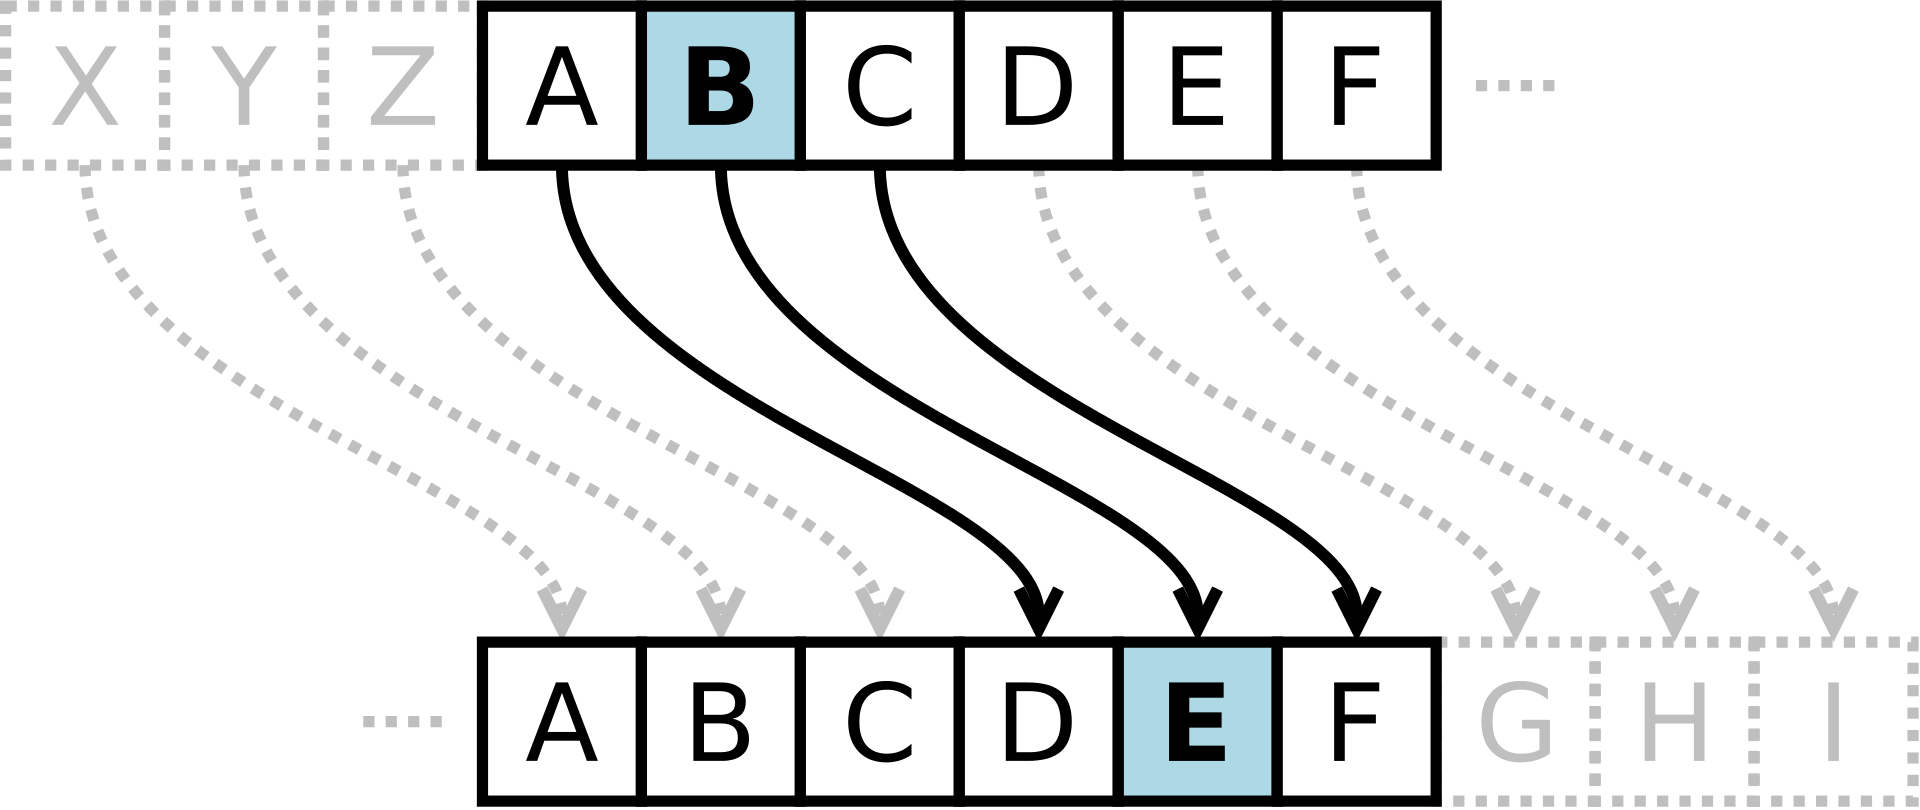
\includegraphics[scale=0.1]{Zesar_zifratu.png}

    \begin{itemize}
        \item \textbf{Jatorrizko alfabetoa}: abcdefghijklmnñopqrstuvwxyz
        \item \textbf{Alfabeto zifratua}: defghijklmnñopqrstuvwxyzabc
    \end{itemize}
\end{itemize}





\chapter{Inplementatutako funtzioen kodea}
\section{zkh 1.bertsioa}
\begin{verbatim}
    # Bi zenbaki oso emanik, a eta b, zatitzaile komunetako handiena 
    # kalkulatuko duen funtzioaren inplementazioa Euklidesen algoritmoan
    # oinarrituz:
    zkh <- function(a,b){ 
        c<-a;
        d<-b;
        while (d != 0) {
            r=mod(c,d);
            c=d;
            d=r;
        }
        return(c)  
    }
\end{verbatim}

\newpage
\subsection{Deiak funtzioari}
\begin{verbatim}
    > zkh(2689,4001)
    [1] 1
    > zkh(1369,2597)
    [1] 1
    > zkh(3.2,4)
    Error in mod(c, d) : 
    Arguments 'n', 'm' must be integers or vectors of integers. 
    > zkh("a","b")
     Error in mod(c, d) : is.numeric(n) is not TRUE 
\end{verbatim}

\newpage

\section{zkh 2.bertsioa}
\begin{verbatim}
    # Parametro moduan jasotako a,b Euklidesen algoritmoan oinarrituz
    # zatitzaile komunetako handiena itzuliko du
    # Parametro moduan zenbaki errealak pasaz gero, errore
    # mezua erakutsiz, karaktereak pasaz gero, baita.
    zkh <- function(a,b){ 
        if(is.character(a)==FALSE & is.character(b)==FALSE){
            c=abs(a)
            d=abs(b)
            if(isNatural(c)&isNatural(d)){
                c<-a;
                d<-b;
                while (d != 0) {
                    r=mod(c,d);
                    c=d;
                    d=r;
                }
                return(c)
            }
            else{
                print('a eta b parametroak zenbaki osoak izan behar dute.')
            }
        }
        else{  
            print('a eta b ezin dira karaktereak izan.')
        }
    }
\end{verbatim}

\newpage

\subsection{Deiak funtzioari}
\begin{verbatim}
    > zkh(231,1820)
    [1] 7
    > zkh(1369,2597)
    [1] 1
    > zkh(3.2,4)
    [1] "a eta b parametroak zenbaki osoak izan behar dute." 
    > zkh(5,'b')
    [1] "a eta b ezin dira karaktereak izan."
\end{verbatim}

\newpage
\section{lehen\_erlatibo\_txiki}
\begin{verbatim}
    # Parametro moduan funtzioari pasatako m-rekin lehen erlatiboa 
    # den zenbaki oso positiborik txikiena itzuliko du
    # RSA_gakoak funtzioa inplementatzeko erabiliko dugu
    lehen_erlatibo_txiki <- function(m){
        zk = 2
        while (GCD(m, zk) != 1){
            zk = zk + 1;
        }
        return(zk);
    }
\end{verbatim}

\subsection{Deiak funtzioari}
\begin{verbatim}
    > lehen_erlatibo_txiki(13797)
    [1] 2
    > # 2
    > lehen_erlatibo_txiki(16974)
    [1] 5
    > # 5
    > lehen_erlatibo_txiki(56970)
    [1] 7
    > # 7
    > lehen_erlatibo_txiki(1000000000000000)
    [1] 3
\end{verbatim}
    
\newpage

\section{RSA\_gakoak}
\begin{verbatim}
    # Bi zenbaki lehen emanik, p eta q, n, r eta s kalkulatuko 
    # ditu, eta irteera estandarretik inprimatu. r txikia kalkulatuko
    # da.
    RSA_gakoak <- function(p,q){
        n = p * q;
        m = (p - 1) * (q - 1);
        r = lehen_erlatibo_txiki(m);
        s = modinv(r, m);
        cat("n = ", n, ", r = ", r, ", s = ", s); 
    }
\end{verbatim}
\subsection{Deiak funtzioari}
\begin{verbatim}
    > RSA_gakoak(5,17)
    n =  85 , r =  3 , s =  43
    > RSA_gakoak(17,23)
    n =  391 , r =  3 , s =  235
    > RSA_gakoak(97,101)
    n =  9797 , r =  7 , s =  2743
    > RSA_gakoak(307,397)
    n =  121879 , r =  5 , s =  96941
\end{verbatim}

\newpage

\section{kodetu}
\begin{verbatim}
    # Parametro moduan txt karaktere string-a jaso eta dagozkion  
    # ASCII kodeak itzultzen ditu.
    kodetu <- function(txt){
        return(strtoi(charToRaw(txt), 16L));
    }
\end{verbatim}

\subsection{Deiak funtzioari}
\begin{verbatim}
    # Ondoren, deskodetu funtzioarekin konprobatuko dugu  
    # ondo kodetu direla
    > testu1<-"kaixo"
    > kodebektore1<-kodetu(testu1)
    > kodebektore1
    [1] 107  97 105 120 111
    > testu2<-"KAIXO"
    > kodebektore2<-kodetu(testu2)
    > kodebektore2
    [1] 75 65 73 88 79
    > testu3<-"Zer moduz?"
    > kodebektore3<-kodetu(testu3)
    > kodebektore3
     [1]  90 101 114  32 109 111 100 117 122  63
\end{verbatim}

\newpage

\section{deskodetu}
\begin{verbatim}
    # Parametro moduan ASCII kodeak jaso eta dagokion txt karaktere 
    # string-a itzultzen duen funtzioa.
    deskodetu <- function(kodetxt){
        return(rawToChar(as.raw(kodetxt)));
    }   
\end{verbatim}

\subsection{Deiak Funtzioari}
\begin{verbatim}
    # Kodetu funtzioarekin kodetutatko bektoreak 
    # deskodetuko ditugu
    > txt1<-deskodetu(kodebektore1)
    > txt1
    [1] "kaixo"
    > txt2<-deskodetu(kodebektore2)
    > txt2
    [1] "KAIXO"
    > txt3<-deskodetu(kodebektore3)
    > txt3
    [1] "Zer moduz?"
\end{verbatim}

\newpage

\section{zifratu}
\begin{verbatim}
    # Parametro moduan ASCII kodeez osatutako bektore bat jaso eta 
    # dagokion bektore zifratua itzuliko du
    zifratu <- function(kodebektorea,r,n){
        luzeera = length(kodebektorea);
        for (i in 1:luzeera)
        {
            kodebektorea[i] = modpower(kodebektorea[i], r, n);
        }
        return(kodebektorea);
    }
\end{verbatim}

\subsection{Deiak funtzioari}
\begin{verbatim}
    > # Erabiliko ditugun gakoak:
    > # n=9797, r=7, s=2743
    > bektorezifratu1<-zifratu(kodebektore1,7,9797)
    > bektorezifratu1
    [1] 2792 5432 4668 4973 7969
    > bektorezifratu2<-zifratu(kodebektore2,7,9797)
    > bektorezifratu2
    [1] 7976 4764 2565 8540 4974
    > bektorezifratu3<-zifratu(kodebektore3,7,9797)
    > bektorezifratu3
     [1]  375 2222 7721 3675  493 7969 6261 8564 4122 4604
\end{verbatim}

\newpage

\section{deszifratu}
\begin{verbatim}
    # Parametro moduan bektore zifratu bat jaso eta dagozkion 
    # ASCII kodeak itzuliko du
    deszifratu <- function(bektorezifratu,s,n){
        luzeera = length(bektorezifratu);
        for (i in 1:luzeera)
        {
            bektorezifratu[i] = modpower(bektorezifratu[i], s, n);
        }
      return(bektorezifratu);
    }
\end{verbatim}

\subsection{Deiak funtzioari}
\begin{verbatim}
    > # RSA_gakoak(97,101) zenbaki lehenetatik lortutako gakoekin:
    > # n=9797, r=7, s=2743
    > n<-9797
    > r<-7
    > s<-2743
    > testuberria<-"ea hau ondo doan..."
    > testuberri_zifratua <- zifratu(kodetu(testuberria),r,n)
    > testuberri_zifratua
     [1] 2222 5432 3675 1177 5432 8564 3675 7969 9305 6261
    [11] 7969 3675 6261 7969 5432 9305 3037 3037 3037
    > testuberri_errekuperatua <- deskodetu(deszifratu(testuberri_zifratua,s,n))
    > testuberri_errekuperatua
    [1] "ea hau ondo doan..."
\end{verbatim}

\chapter{Bibliografia}



\chapter{Iritzi pertsonala}




\end {document}